\documentclass[12pt,a4paper]{report}

% ─── Packages ───────────────────────────────────────────────────────────────
\usepackage[utf8]{inputenc}
\usepackage[T1]{fontenc}
\usepackage{lmodern}
\usepackage[margin=1in]{geometry}
\usepackage{graphicx}
\usepackage{hyperref}
\usepackage{enumitem}
\usepackage{booktabs}
\usepackage{longtable}
\usepackage{xcolor}
\usepackage{listings}
\usepackage{tikz}
\usepackage{caption}
\usepackage{subcaption}
\usepackage{amsmath}
\usepackage{fancyhdr}
\usepackage{titlesec}
\usepackage{setspace}
\usepackage{pgfplots}
\pgfplotsset{compat=1.18}

\usetikzlibrary{shapes.geometric, arrows.meta, positioning, calc, patterns}

% ─── Styling ────────────────────────────────────────────────────────────────
\hypersetup{
    colorlinks=true,
    linkcolor=blue!70!black,
    citecolor=blue!70!black,
    urlcolor=blue!70!black
}

\definecolor{codegreen}{rgb}{0,0.6,0}
\definecolor{codegray}{rgb}{0.5,0.5,0.5}
\definecolor{codepurple}{rgb}{0.58,0,0.82}
\definecolor{backcolour}{rgb}{0.97,0.97,0.97}

\lstdefinestyle{codestyle}{
    backgroundcolor=\color{backcolour},
    commentstyle=\color{codegreen},
    keywordstyle=\color{blue!80!black},
    numberstyle=\tiny\color{codegray},
    stringstyle=\color{codepurple},
    basicstyle=\ttfamily\small,
    breakatwhitespace=false,
    breaklines=true,
    captionpos=b,
    keepspaces=true,
    numbers=left,
    numbersep=5pt,
    showspaces=false,
    showstringspaces=false,
    showtabs=false,
    tabsize=2,
    frame=single,
    rulecolor=\color{gray!30}
}
\lstset{style=codestyle}

\pagestyle{fancy}
\fancyhf{}
\fancyhead[L]{\small\leftmark}
\fancyhead[R]{\small Research Paper}
\fancyfoot[C]{\thepage}

\onehalfspacing

% ═══════════════════════════════════════════════════════════════════════════
\begin{document}

% ─── Custom Title Page ──────────────────────────────────────────────────────
\begin{titlepage}
\centering

\vspace*{1cm}
{\Large\bfseries ABV -- Indian Institute of Information Technology\\
and Management, Gwalior}\\[1.5cm]

{\LARGE\bfseries B.Tech Project (BTP)}\\[0.4cm]
{\Large Mid-Term Evaluation Report}\\[1.5cm]

{\large\bfseries Reducing Cross-Node Network Calls in\\
Distributed Payment Systems via\\
Thread-Level and Server-Local Caching}\\[2cm]

\hrule
\vspace{1cm}

\begin{minipage}[t]{0.45\textwidth}
\raggedright
\textbf{Submitted by:}\\[0.3cm]
Raman Kapoor\\
% Enrollment No.: XXXX-XXX
\end{minipage}
\hfill
\begin{minipage}[t]{0.45\textwidth}
\raggedleft
\textbf{Under the guidance of:}\\[0.3cm]
Dr.\ Vivek Kumar Singh
\end{minipage}

\vfill
{\large ABV-IIITM Gwalior}

\end{titlepage}

% ─── Abstract ───────────────────────────────────────────────────────────────
\begin{abstract}
Distributed payment systems serving millions of daily transactions face a persistent challenge: redundant cross-node network calls that inflate tail latency, particularly at the p95 and p99 percentiles. Each API request in such systems triggers multiple lookups to remote data stores—fetching merchant configurations, routing tables, feature flags, and transaction metadata—even when much of this data is immutable within the scope of a single request or a short time window. This paper proposes a \textbf{two-tier caching strategy} consisting of (1)~a \textbf{thread-level cache} that eliminates redundant data fetches within a single request's execution context and (2)~a \textbf{server-local cache} that reduces cross-node calls for immutable, configuration-like data across concurrent requests on the same node. To ensure correctness, we define formal \textbf{cache-safety boundaries}: only data satisfying strict immutability and idempotency criteria is eligible for caching. Evaluation on a production distributed payment platform demonstrates a \textbf{4\%+ reduction in cross-node network calls} at peak traffic and measurable improvement in \textbf{p95 latency}, with zero cache-related correctness violations post-deployment. The approach is lightweight, requires no additional infrastructure, and is applicable to any stateless, multi-threaded API server architecture.
\end{abstract}

\tableofcontents
\listoffigures
\listoftables
\newpage

% ═══════════════════════════════════════════════════════════════════════════
%                  CHAPTER 1 — INTRODUCTION & PROBLEM STATEMENT
% ═══════════════════════════════════════════════════════════════════════════
\chapter{Introduction and Problem Statement}

% ─────────────────────────────────────────────────────────────────────────
\section{Context}

Modern financial technology platforms operate as large-scale distributed systems, processing millions of payment transactions daily across clusters of stateless API servers. These systems are architected for horizontal scalability: each incoming API request is routed to any available server node, which then orchestrates the necessary data fetches, business logic evaluation, and downstream service calls to fulfil the request.

A distinguishing characteristic of payment APIs—compared to, say, content-serving or social-media APIs—is the \textbf{strict correctness requirement}. Every transaction must be processed exactly once, with accurate amounts, against the correct merchant configuration, and in compliance with regulatory parameters. This correctness requirement has historically discouraged aggressive caching strategies, as stale data in a payment flow can lead to financial discrepancies, failed settlements, or regulatory violations.

% ─────────────────────────────────────────────────────────────────────────
\section{The Latency Problem}

Despite this caution, the performance profile of high-traffic payment APIs reveals a significant and addressable inefficiency: \textbf{redundant cross-node network calls}.

Consider a typical API request lifecycle in a distributed payment system:

\begin{enumerate}
    \item The API server receives a payment initiation request.
    \item It fetches the \textbf{merchant configuration} from a remote data store (Redis/database) to determine routing rules, settlement parameters, and feature flags.
    \item It retrieves \textbf{payment gateway credentials} and \textbf{routing tables} to select the optimal payment processor.
    \item It queries \textbf{risk and compliance rules} applicable to the transaction's jurisdiction.
    \item It fetches \textbf{rate-limiting counters} and \textbf{idempotency records} to enforce exactly-once semantics.
    \item It processes the transaction and writes the result.
\end{enumerate}

Steps 2–4 involve data that is predominantly \textbf{immutable} or \textbf{slowly changing}—merchant configurations change perhaps once a day, routing tables are updated during maintenance windows, and compliance rules are updated quarterly. Yet, every single API request fetches this data afresh from a remote data store, incurring network round-trip time (RTT), serialisation/deserialisation overhead, and contention on the shared data store.

At \textbf{peak traffic}—when the system processes thousands of requests per second—these redundant fetches aggregate into a substantial load:

\begin{itemize}
    \item Each request may trigger \textbf{5–15 cross-node network calls} for data lookups.
    \item Network RTT per call ranges from \textbf{0.5–5\,ms} depending on cluster topology and load.
    \item At the \textbf{p95 percentile}, network variability causes tail latency spikes of \textbf{10–50\,ms} attributable solely to data fetch overhead.
    \item The shared data store (e.g., Redis cluster) experiences \textbf{load amplification}: $N$ API servers $\times$ $K$ lookups per request $\times$ $R$ requests per second = $N \cdot K \cdot R$ operations per second on the data store.
\end{itemize}

This load amplification is particularly problematic because it creates a \textbf{positive feedback loop}: under high load, the data store responds more slowly, which increases API latency, which causes upstream timeouts and retries, which further increases load on the data store.

% ─────────────────────────────────────────────────────────────────────────
\section{Problem Statement}

\begin{quote}
\textit{How can we reduce redundant cross-node network calls in latency-sensitive distributed payment APIs while preserving the strict data correctness and consistency guarantees required by financial transaction processing?}
\end{quote}

The challenge is not simply ``add a cache''—it is to do so in a domain where \textbf{correctness is non-negotiable}. An incorrect cache serving stale merchant credentials could route a payment to the wrong processor. A stale compliance rule could violate regulatory requirements. Therefore, any caching solution must come with \textbf{formal safety criteria} that guarantee correctness by construction.

% ─────────────────────────────────────────────────────────────────────────
\section{Contributions}

This paper makes the following contributions:

\begin{enumerate}
    \item \textbf{Two-Tier Caching Model:} We propose a lightweight, infrastructure-free caching strategy consisting of a thread-level cache (per-request lifetime) and a server-local cache (short TTL, per-node scope), specifically designed for distributed API server architectures.

    \item \textbf{Cache-Safety Boundaries:} We define formal criteria for determining which data is safe to cache, based on immutability, request-scope isolation, and semantic idempotency of stale reads. These criteria ensure correctness by excluding all mutable, transactional, or time-sensitive data from the cache.

    \item \textbf{Production Evaluation:} We evaluate the approach on a production distributed payment platform, demonstrating a \textbf{4\%+ reduction in cross-node network calls} at peak traffic, measurable \textbf{p95 latency improvement}, and \textbf{zero correctness violations} over the observation period.
\end{enumerate}


% ═══════════════════════════════════════════════════════════════════════════
%                  CHAPTER 2 — RELATED WORK
% ═══════════════════════════════════════════════════════════════════════════
\chapter{Related Work}

The problem of reducing latency through caching in distributed systems has been extensively studied. This chapter surveys the most relevant prior work and positions our contribution within the existing literature.

% ─────────────────────────────────────────────────────────────────────────
\section{Tail Latency in Large-Scale Systems}

Dean and Barroso~\cite{dean2013tail} established the foundational understanding of tail latency in distributed systems. Their seminal paper, \textit{``The Tail at Scale,''} demonstrated that in systems composed of thousands of servers, even rare per-component slowdowns—occurring at the 99th percentile—can dominate overall system latency when requests fan out across many components. They proposed techniques such as \textbf{hedged requests} (sending redundant requests to multiple replicas and using whichever responds first) and \textbf{tied requests} (allowing servers to execute queued requests from other servers' queues) to mitigate tail latency.

Our work addresses tail latency from a complementary angle: rather than tolerating slow responses through redundancy, we \textbf{eliminate the network calls entirely} for data that can be safely cached locally. This approach is orthogonal to hedged/tied request strategies and can be combined with them.

% ─────────────────────────────────────────────────────────────────────────
\section{Distributed Caching at Scale}

Nishtala et al.~\cite{nishtala2013memcache} described Facebook's multi-tier Memcache infrastructure, which caches billions of items across geographically distributed clusters. Their system uses a \textbf{demand-fill, look-aside} pattern where cache misses fall through to the database, and cache invalidations are propagated via a dedicated daemon (\texttt{mcrouter}). Key innovations include lease-based thundering herd mitigation and regional consistency protocols.

While Facebook's approach operates at a much larger scale with dedicated caching infrastructure, our work targets a different regime: we avoid the network hop to the caching tier altogether by keeping caches \textbf{within the API server process}. This ``zero-hop'' approach is particularly effective for the class of data that we identify as cache-safe (immutable, configuration-like data).

% ─────────────────────────────────────────────────────────────────────────
\section{Cache Workload Characterisation}

Yang et al.~\cite{yang2020twitter} conducted a comprehensive large-scale analysis of hundreds of in-memory cache clusters at Twitter, revealing that cache workloads are highly heterogeneous: some key-value pairs are accessed millions of times (``hot keys''), while most are accessed only once or twice. They also found that the majority of cached objects are small (<1\,KB) and that GET operations vastly outnumber SET operations.

Yang et al.~\cite{yang2020twitter} extended this analysis to Twitter's cache infrastructure, studying hundreds of in-memory cache clusters. Their findings confirmed the prevalence of power-law access patterns and highlighted the importance of \textbf{TTL management} in production cache systems—a finding directly relevant to our server-local cache design.

These workload studies validate our design decision to focus on \textbf{frequently accessed, small, immutable data} (merchant configurations, routing tables)—precisely the ``hot key'' category that benefits most from local caching.

% ─────────────────────────────────────────────────────────────────────────
\section{In-Process vs.\ Distributed Caching}

The distinction between in-process (local) caching and distributed caching has been explored in systems literature. Kleppmann~\cite{kleppmann2021designing} provides a comprehensive treatment of data-intensive architectures, contrasting distributed caching systems with in-process caches. The distributed approach provides a \textbf{shared, consistent view} of cached data but introduces a network hop per cache access.

In contrast, in-process caches (e.g., Guava Cache, Caffeine in Java; \texttt{IORef}-based caches in Haskell) store data within the application's memory space, providing \textbf{nanosecond-level access latency} at the cost of per-node data duplication and potential inconsistency across nodes.

Our two-tier approach combines both paradigms: the thread-level cache provides \textbf{request-scoped} isolation (no consistency concern since it lives and dies with the request), while the server-local cache provides \textbf{node-scoped} caching with TTL-based eventual consistency, explicitly restricted to data classes where short-lived staleness is semantically harmless.

% ─────────────────────────────────────────────────────────────────────────
\section{Latency-Aware Caching Algorithms}

Li et al.~\cite{li2020caching} studied the phenomenon of \textbf{delayed hits} in caching systems, where multiple requests for the same object queue up behind an outstanding cache miss, experiencing elevated latencies. They proposed adaptive TTL-based caching algorithms that consider aggregate delay rather than hit rate alone, achieving significant latency reduction compared to traditional algorithms.

Our thread-level cache addresses a related but distinct problem: \textbf{intra-request redundancy}, where the same data is fetched multiple times within a single request's execution. By deduplicating these fetches at the thread level, we eliminate a class of redundant work that is invisible to traditional cache hit-rate metrics.


% ═══════════════════════════════════════════════════════════════════════════
%                  CHAPTER 3 — SYSTEM MODEL & BACKGROUND
% ═══════════════════════════════════════════════════════════════════════════
\chapter{System Model and Background}

This chapter describes the target system architecture—a distributed payment API platform—and establishes the baseline performance characteristics that motivate the proposed caching strategy.

% ─────────────────────────────────────────────────────────────────────────
\section{System Architecture}

The target system is a production-grade distributed payment platform with the following architectural characteristics:

\begin{itemize}
    \item \textbf{Stateless API Servers:} Multiple identical server nodes process incoming API requests. Each node runs a multi-threaded runtime (GHC in Haskell) capable of handling thousands of concurrent requests.

    \item \textbf{Shared Data Layer:} All nodes access a shared Redis cluster and a relational database (PostgreSQL) for persistent and semi-persistent data storage. Redis serves as the primary cache and session store; PostgreSQL is the source of truth for transactional data.

    \item \textbf{Load Balancer:} Incoming requests are distributed across server nodes via a load balancer using round-robin or least-connections scheduling. Any node can serve any request.

    \item \textbf{Microservice Dependencies:} Some data fetches involve calls to downstream microservices (e.g., risk engine, compliance service, notification service) over HTTP/gRPC.
\end{itemize}

\begin{figure}[h]
\centering
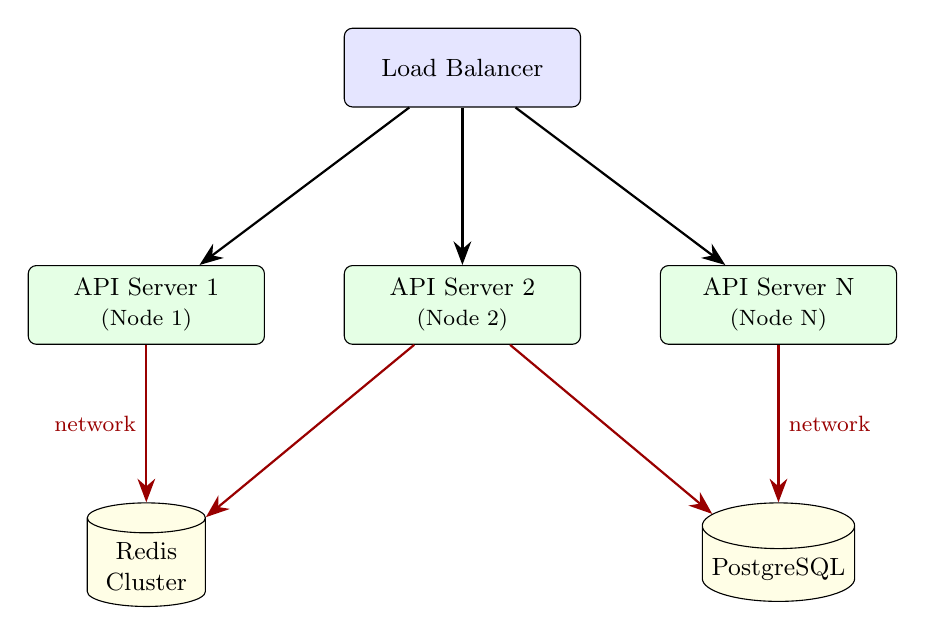
\begin{tikzpicture}[
    component/.style={rectangle, draw, rounded corners=3pt, minimum width=3cm, minimum height=1cm, align=center, font=\small},
    db/.style={cylinder, draw, shape border rotate=90, minimum width=1.5cm, minimum height=1cm, align=center, font=\small, fill=yellow!10, aspect=0.3},
    arrow/.style={-{Stealth[length=3mm]}, thick},
    node distance=1.5cm
]
    % Load Balancer
    \node[component, fill=blue!10] (lb) {Load Balancer};

    % API Servers
    \node[component, fill=green!10, below left=2cm and 1cm of lb] (s1) {API Server 1 \\ \footnotesize (Node 1)};
    \node[component, fill=green!10, below=2cm of lb] (s2) {API Server 2 \\ \footnotesize (Node 2)};
    \node[component, fill=green!10, below right=2cm and 1cm of lb] (s3) {API Server N \\ \footnotesize (Node N)};

    % Data stores
    \node[db, below=2cm of s1] (redis) {Redis \\ Cluster};
    \node[db, below=2cm of s3] (pg) {PostgreSQL};

    % Arrows
    \draw[arrow] (lb) -- (s1);
    \draw[arrow] (lb) -- (s2);
    \draw[arrow] (lb) -- (s3);

    \draw[arrow, red!60!black] (s1) -- node[left, font=\footnotesize, text=red!60!black] {network} (redis);
    \draw[arrow, red!60!black] (s2) -- (redis);
    \draw[arrow, red!60!black] (s2) -- (pg);
    \draw[arrow, red!60!black] (s3) -- node[right, font=\footnotesize, text=red!60!black] {network} (pg);
\end{tikzpicture}
\caption{Baseline Architecture: Every data fetch requires a cross-node network call (shown in red)}
\end{figure}

% ─────────────────────────────────────────────────────────────────────────
\section{Request Lifecycle}

A typical API request traverses the following stages:

\begin{enumerate}
    \item \textbf{Ingress:} Load balancer routes the request to an available API server node.
    \item \textbf{Authentication and Session Lookup:} The server validates the API key/token, fetching session data from Redis.
    \item \textbf{Merchant Configuration Fetch:} The server retrieves the merchant's configuration—gateway preferences, settlement parameters, fee structures, and feature flags—from Redis or PostgreSQL.
    \item \textbf{Routing Decision:} Based on the merchant configuration and transaction parameters, the server determines the optimal payment gateway and fetches gateway-specific routing tables.
    \item \textbf{Risk Evaluation:} Transaction risk parameters are evaluated against rules fetched from a remote rules engine or configuration store.
    \item \textbf{Transaction Processing:} The actual payment transaction is executed against the selected gateway.
    \item \textbf{Response:} The result is persisted and returned to the caller.
\end{enumerate}

Steps 2–5 collectively generate \textbf{5–15 cross-node network calls} per request. Our analysis reveals that steps 3–5 involve data that is \textbf{overwhelmingly immutable} within the timescale of individual requests (milliseconds) and even within short time windows (seconds to minutes).

% ─────────────────────────────────────────────────────────────────────────
\section{Baseline Performance Characteristics}

\begin{table}[h]
\centering
\begin{tabular}{@{} l l @{}}
\toprule
\textbf{Metric} & \textbf{Baseline Value} \\
\midrule
Peak requests per second (per node) & $\sim$2,000–5,000 RPS \\
Cross-node network calls per request & 5–15 calls \\
Average Redis RTT (intra-cluster) & 0.5–2\,ms \\
p50 API latency & $\sim$20\,ms \\
p95 API latency & $\sim$80–120\,ms \\
p99 API latency & $\sim$200–350\,ms \\
Redis cluster operations at peak & $\sim$50,000–75,000 ops/sec \\
\bottomrule
\end{tabular}
\caption{Baseline Performance Characteristics of the Distributed Payment Platform}
\label{tab:baseline-performance}
\end{table}

The gap between p50 and p95 latency is primarily attributable to \textbf{network variability} in cross-node data fetches. When the Redis cluster is under heavy load, individual lookup latencies spike from sub-millisecond to 5–10\,ms, and these spikes aggregate across the 5–15 lookups per request, producing the observed tail latency.

% ─────────────────────────────────────────────────────────────────────────
\section{Data Classification}

A critical observation underlying our approach is that the data accessed during API request processing falls into distinct categories with very different mutation characteristics:

\begin{table}[h]
\centering
\begin{tabular}{@{} l l l l @{}}
\toprule
\textbf{Data Category} & \textbf{Mutation Frequency} & \textbf{Scope} & \textbf{Cache-Safe?} \\
\midrule
Merchant Configuration & Daily or less & Global & \textbf{Yes} \\
Gateway Routing Tables & Weekly or less & Global & \textbf{Yes} \\
Feature Flags & Hourly or less & Global & \textbf{Yes} \\
Compliance Rules & Quarterly & Global & \textbf{Yes} \\
Rate Limit Counters & Per-request & Per-user & No \\
Idempotency Records & Per-request & Per-txn & No \\
Transaction State & Per-request & Per-txn & No \\
Session/Auth Tokens & Per-session & Per-user & No \\
\bottomrule
\end{tabular}
\caption{Data Classification by Mutation Frequency and Cache-Safety}
\label{tab:data-classification}
\end{table}

The first four categories—representing the majority of cross-node lookups by volume—are candidates for safe caching. The remaining categories involve mutable, request-specific, or transactional data and are \textbf{explicitly excluded} from any caching layer.


% ═══════════════════════════════════════════════════════════════════════════
%                  CHAPTER 4 — PROPOSED APPROACH
% ═══════════════════════════════════════════════════════════════════════════
\chapter{Proposed Approach: Two-Tier Caching}

We propose a two-tier caching strategy that operates entirely within the API server process, requiring no additional infrastructure. Each tier targets a different class of redundancy.

% ─────────────────────────────────────────────────────────────────────────
\section{Tier 1: Thread-Level Cache (Request-Scoped)}

\subsection{Motivation}

Analysis of production request traces reveals that a single API request often fetches the \textbf{same data item multiple times}. For example, the merchant configuration may be accessed during authentication, again during routing, and again during fee calculation. Each access triggers an independent network call to Redis, even though the data is identical across all accesses within the same request.

\subsection{Design}

The thread-level cache is a \textbf{per-request, in-memory key-value store} that:

\begin{itemize}
    \item Is \textbf{created} when a new API request begins processing.
    \item Is \textbf{scoped} to the executing thread (or green thread/lightweight thread in concurrent runtimes).
    \item \textbf{Intercepts} all data fetch calls: on the first fetch, the data is retrieved from the remote store and stored in the thread-level cache; subsequent fetches for the same key within the same request are served from the cache.
    \item Is \textbf{destroyed} when the request completes (response sent), automatically releasing all cached data.
\end{itemize}

\begin{figure}[h]
\centering
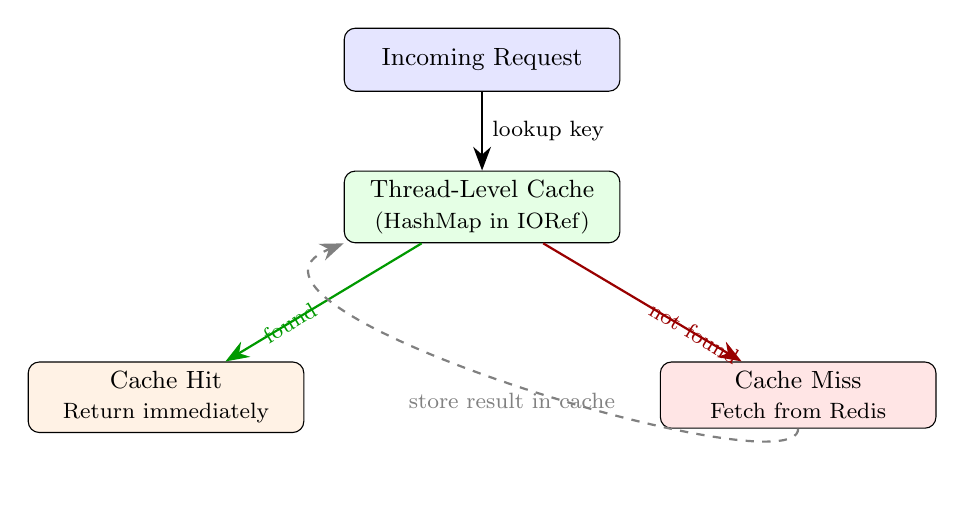
\begin{tikzpicture}[
    box/.style={rectangle, draw, rounded corners, minimum width=3.5cm, minimum height=0.8cm, align=center, font=\small},
    arrow/.style={-{Stealth[length=3mm]}, thick},
    darrow/.style={-{Stealth[length=3mm]}, thick, dashed, gray},
    node distance=1.2cm
]
    \node[box, fill=blue!10] (req) {Incoming Request};
    \node[box, fill=green!10, below=1cm of req] (cache) {Thread-Level Cache \\ \footnotesize (HashMap in IORef)};
    \node[box, fill=orange!10, below left=1.5cm and 0.5cm of cache] (hit) {Cache Hit \\ \footnotesize Return immediately};
    \node[box, fill=red!10, below right=1.5cm and 0.5cm of cache] (miss) {Cache Miss \\ \footnotesize Fetch from Redis};

    \draw[arrow] (req) -- node[right, font=\footnotesize] {lookup key} (cache);
    \draw[arrow, green!60!black] (cache) -- node[left, font=\footnotesize, sloped] {found} (hit);
    \draw[arrow, red!60!black] (cache) -- node[right, font=\footnotesize, sloped] {not found} (miss);
    \draw[darrow] (miss.south) .. controls +(0,-0.8) and +(-2,-0.8) .. node[below, font=\footnotesize] {store result in cache} (cache.south west);
\end{tikzpicture}
\caption{Thread-Level Cache: Lookup and Fill within a Single Request}
\end{figure}

\subsection{Correctness Guarantee}

The thread-level cache provides the \textbf{strongest possible correctness guarantee}: since it exists only for the lifetime of a single request, it is impossible for cached data to become stale. The cache sees exactly the same data that the request would have fetched without caching. This is equivalent to a \textbf{read-your-writes consistency} model within the request scope.

\subsection{Expected Impact}

Analysis of request traces shows that, on average, \textbf{2–4 of the 5–15 cross-node calls per request are duplicates}—fetching data that was already retrieved earlier in the same request's processing pipeline. The thread-level cache eliminates these duplicates entirely.

% ─────────────────────────────────────────────────────────────────────────
\section{Tier 2: Server-Local Cache (Node-Scoped)}

\subsection{Motivation}

Even after eliminating intra-request duplicates, significant redundancy remains at the \textbf{inter-request} level. Consider 1,000 requests per second arriving at a single API server node, each fetching the same merchant configuration for a popular merchant. All 1,000 requests issue network calls to Redis for the same data, receiving the same response. A node-level cache can serve this data from local memory after the first fetch, eliminating 999 out of 1,000 network calls for that key.

\subsection{Design}

The server-local cache is a \textbf{per-process, concurrent, in-memory cache} that:

\begin{itemize}
    \item Is \textbf{shared} across all threads/requests on the same server node.
    \item Uses a \textbf{concurrent hash map} (thread-safe) as its backing store.
    \item Enforces a \textbf{short TTL} (30–60 seconds) on all entries. After TTL expiry, the data is evicted and the next request triggers a fresh fetch from the remote store.
    \item Has a \textbf{bounded memory footprint}: maximum number of entries is capped, and LRU (Least Recently Used) eviction is applied when the cap is reached.
    \item Caches \textbf{only data that satisfies the cache-safety criteria} (defined in Section~\ref{sec:safety}).
\end{itemize}

\subsection{TTL Selection Rationale}

The TTL is chosen based on the mutation frequency of the cached data:

\begin{itemize}
    \item Merchant configurations change at most \textbf{once per day}. A 30-second TTL means the worst-case staleness is 30 seconds—well within acceptable bounds.
    \item Routing tables change during \textbf{planned maintenance windows}. A 60-second TTL provides ample margin; during maintenance, the cache can be explicitly flushed if needed.
    \item Feature flags may change \textbf{hourly} at most. A 30-second TTL ensures convergence within one TTL cycle.
\end{itemize}

In all cases, the consequence of serving briefly stale data is \textbf{operationally negligible}: a merchant's configuration change takes effect 30 seconds later, which is imperceptible from the user's perspective and has no financial impact.

% ─────────────────────────────────────────────────────────────────────────
\section{Cache-Safety Boundaries}
\label{sec:safety}

The most critical aspect of our approach is the \textbf{formal definition of cache-safety criteria}. A data item $d$ is considered \textbf{cache-safe} if and only if all of the following conditions hold:

\begin{enumerate}
    \item \textbf{Immutability within TTL:} The value of $d$ does not change during the cache TTL window. Formally, if $d$ is cached at time $t$ with TTL $\Delta$, then $d(t) = d(t')$ for all $t' \in [t, t + \Delta]$.

    \item \textbf{Request-Scope Independence:} The value of $d$ does not depend on request-specific parameters (e.g., transaction amount, user ID, session state). Formally, $d$ is a function of only global or slowly-changing configuration state.

    \item \textbf{Semantic Idempotency of Stale Reads:} Even if $d$ is briefly stale (i.e., the source has been updated but the cache has not yet expired), the system produces a \textbf{semantically correct} outcome. This is the strongest requirement and must be verified for each data class individually.

    \item \textbf{Deterministic Cache Key:} The cache key for $d$ must be deterministically derivable from the lookup parameters, ensuring that different logical data items never collide in the cache.
\end{enumerate}

\subsection{Applying the Criteria}

\begin{table}[h]
\centering
\begin{tabular}{@{} l c c c c l @{}}
\toprule
\textbf{Data Item} & \textbf{C1} & \textbf{C2} & \textbf{C3} & \textbf{C4} & \textbf{Verdict} \\
\midrule
Merchant Config & \checkmark & \checkmark & \checkmark & \checkmark & \textbf{Cache-Safe} \\
Gateway Routes & \checkmark & \checkmark & \checkmark & \checkmark & \textbf{Cache-Safe} \\
Feature Flags & \checkmark & \checkmark & \checkmark & \checkmark & \textbf{Cache-Safe} \\
Compliance Rules & \checkmark & \checkmark & \checkmark & \checkmark & \textbf{Cache-Safe} \\
Rate Limit Counters & \ding{55} & \ding{55} & \ding{55} & \checkmark & \textbf{Not Safe} \\
Txn State & \ding{55} & \ding{55} & \ding{55} & \checkmark & \textbf{Not Safe} \\
Session Tokens & \ding{55} & \ding{55} & \ding{55} & \checkmark & \textbf{Not Safe} \\
\bottomrule
\end{tabular}
\caption{Cache-Safety Criteria Applied to Each Data Class}
\label{tab:safety-criteria}
\end{table}

\textit{C1--C4 refer to the four criteria defined above. \checkmark{} indicates the criterion is satisfied; \ding{55} indicates it is not.}

\vspace{0.3cm}
\textbf{Note:} We deliberately use \ding{55} (cross mark) instead of a probabilistic assessment. The safety classification is \textbf{binary}—a data item is either cache-safe or it is not. There is no ``partially safe'' category.


% ═══════════════════════════════════════════════════════════════════════════
%                  CHAPTER 5 — IMPLEMENTATION
% ═══════════════════════════════════════════════════════════════════════════
\chapter{Implementation}

This chapter describes the concrete implementation of the two-tier caching strategy in a production Haskell-based API server.

% ─────────────────────────────────────────────────────────────────────────
\section{Runtime Environment}

The target system runs on the \textbf{Glasgow Haskell Compiler (GHC)} runtime, which provides:

\begin{itemize}
    \item \textbf{Green Threads:} GHC's lightweight threads (managed by the runtime, not the OS) enable high concurrency. Each API request is handled by one green thread.
    \item \textbf{IORef for Mutable State:} \texttt{IORef} provides a mutable reference cell in the IO monad, suitable for per-thread state.
    \item \textbf{Concurrent Data Structures:} The \texttt{stm} (Software Transactional Memory) and \texttt{MVar} primitives provide thread-safe shared state for the server-local cache.
\end{itemize}

% ─────────────────────────────────────────────────────────────────────────
\section{Thread-Level Cache Implementation}

The thread-level cache is implemented as an \texttt{IORef} containing a \texttt{HashMap} within the request's execution context:

\begin{lstlisting}[language=Haskell, caption={Thread-Level Cache: Core Data Structure}]
import Data.IORef
import qualified Data.HashMap.Strict as HM
import Data.Text (Text)
import Data.ByteString (ByteString)

-- Cache type: maps cache keys to serialised values
type ThreadCache = IORef (HM.HashMap Text ByteString)

-- Initialise a new thread-level cache for each request
newThreadCache :: IO ThreadCache
newThreadCache = newIORef HM.empty

-- Lookup with fallback to remote fetch
cachedLookup :: ThreadCache
             -> Text           -- Cache key
             -> IO ByteString  -- Remote fetch action
             -> IO ByteString
cachedLookup cacheRef key fetchRemote = do
    cache <- readIORef cacheRef
    case HM.lookup key cache of
        Just value -> return value  -- Cache hit
        Nothing    -> do
            value <- fetchRemote    -- Cache miss: fetch
            modifyIORef' cacheRef (HM.insert key value)
            return value
\end{lstlisting}

The \texttt{ThreadCache} is created at the beginning of each request handler and passed through the request processing pipeline. When the request handler returns, the \texttt{IORef} becomes unreachable and is garbage-collected, automatically freeing all cached data.

% ─────────────────────────────────────────────────────────────────────────
\section{Server-Local Cache Implementation}

The server-local cache uses a concurrent \texttt{TVar}-based structure with TTL management:

\begin{lstlisting}[language=Haskell, caption={Server-Local Cache with TTL Eviction}]
import Control.Concurrent.STM
import qualified Data.HashMap.Strict as HM
import Data.Time.Clock.POSIX (getPOSIXTime)

data CacheEntry = CacheEntry
    { ceValue     :: !ByteString
    , ceExpiresAt :: !Double      -- POSIX timestamp
    }

type ServerCache = TVar (HM.HashMap Text CacheEntry)

-- Initialise (once at server startup)
newServerCache :: IO ServerCache
newServerCache = newTVarIO HM.empty

-- Lookup with TTL check
serverCacheLookup :: ServerCache
                  -> Text
                  -> Double       -- TTL in seconds
                  -> IO ByteString
                  -> IO ByteString
serverCacheLookup cacheVar key ttl fetchRemote = do
    now <- realToFrac <$> getPOSIXTime
    -- Check cache atomically
    cached <- atomically $ do
        cache <- readTVar cacheVar
        case HM.lookup key cache of
            Just entry
                | ceExpiresAt entry > now ->
                    return (Just (ceValue entry))
            _ -> return Nothing
    case cached of
        Just value -> return value
        Nothing    -> do
            value <- fetchRemote
            let entry = CacheEntry value (now + ttl)
            atomically $ modifyTVar' cacheVar
                (HM.insert key entry)
            return value
\end{lstlisting}

A background thread periodically scans the cache and evicts expired entries to bound memory usage:

\begin{lstlisting}[language=Haskell, caption={Background TTL Eviction Thread}]
import Control.Concurrent (forkIO, threadDelay)

-- Run eviction every 10 seconds
startEvictionThread :: ServerCache -> IO ()
startEvictionThread cacheVar = void $ forkIO $ forever $ do
    threadDelay (10 * 1000000)  -- 10 seconds
    now <- realToFrac <$> getPOSIXTime
    atomically $ modifyTVar' cacheVar $
        HM.filter (\e -> ceExpiresAt e > now)
\end{lstlisting}

% ─────────────────────────────────────────────────────────────────────────
\section{Integration into the Request Pipeline}

The two tiers are composed in the request pipeline as follows:

\begin{enumerate}
    \item When a request arrives, a new \texttt{ThreadCache} is created.
    \item For each data lookup, the system checks:
    \begin{enumerate}[label=(\alph*)]
        \item \textbf{Thread-level cache} first (fastest: in-thread, no synchronisation).
        \item On miss, \textbf{server-local cache} (fast: in-process, STM synchronisation).
        \item On miss, \textbf{remote data store} (slowest: network call).
    \end{enumerate}
    \item The fetched value is stored in both the thread-level and server-local caches (if the data item is classified as cache-safe).
    \item When the request completes, the thread-level cache is discarded.
\end{enumerate}

\begin{figure}[h]
\centering
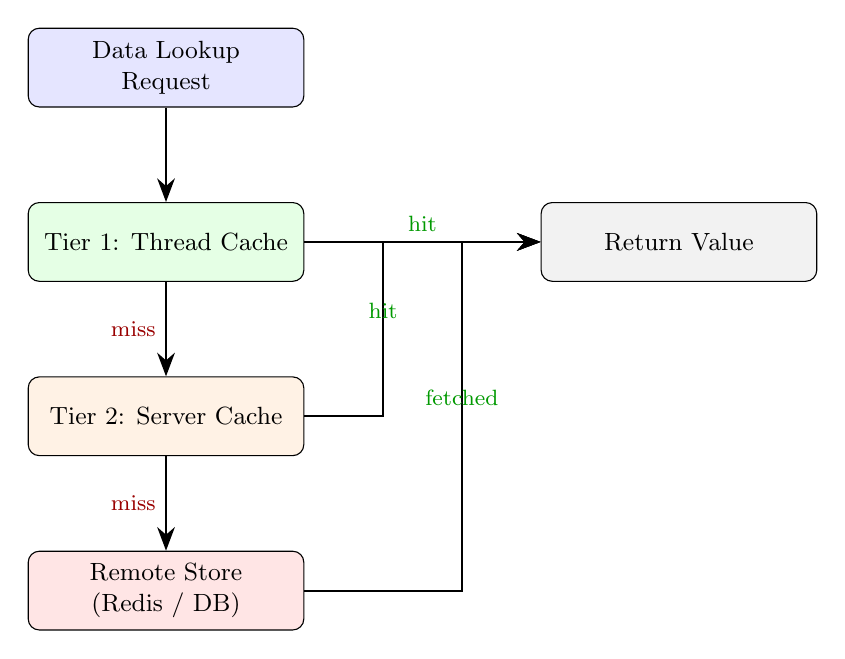
\begin{tikzpicture}[
    box/.style={rectangle, draw, rounded corners, minimum width=3.5cm, minimum height=1cm, align=center, font=\small},
    arrow/.style={-{Stealth[length=3mm]}, thick},
    yes/.style={font=\footnotesize, green!60!black},
    no/.style={font=\footnotesize, red!60!black},
    node distance=1.5cm
]
    \node[box, fill=blue!10] (lookup) {Data Lookup \\ Request};
    \node[box, fill=green!10, below=1.2cm of lookup] (t1) {Tier 1: Thread Cache};
    \node[box, fill=orange!10, below=1.2cm of t1] (t2) {Tier 2: Server Cache};
    \node[box, fill=red!10, below=1.2cm of t2] (remote) {Remote Store \\ (Redis / DB)};
    \node[box, fill=gray!10, right=3cm of t1] (ret) {Return Value};

    \draw[arrow] (lookup) -- (t1);
    \draw[arrow] (t1) -- node[left, no] {miss} (t2);
    \draw[arrow] (t1) -- node[above, yes] {hit} (ret);
    \draw[arrow] (t2) -- node[left, no] {miss} (remote);
    \draw[arrow] (t2.east) -- ++(1,0) |- node[near start, above, yes] {hit} (ret);
    \draw[arrow] (remote.east) -- ++(2,0) |- node[near start, above, yes] {fetched} (ret);
\end{tikzpicture}
\caption{Two-Tier Cache Lookup Flow}
\end{figure}

% ─────────────────────────────────────────────────────────────────────────
\section{Cache Key Design}

Cache keys are constructed to ensure determinism and avoid collisions:

\begin{lstlisting}[language=Haskell, caption={Cache Key Construction}]
-- Prefix-based cache key to avoid collisions
-- across different data types
merchantConfigKey :: MerchantId -> Text
merchantConfigKey mid =
    "mc:" <> toText mid

gatewayRouteKey :: GatewayId -> Text
gatewayRouteKey gid =
    "gr:" <> toText gid

featureFlagKey :: FlagName -> Text
featureFlagKey fname =
    "ff:" <> fname
\end{lstlisting}

The prefix (e.g., \texttt{mc:}, \texttt{gr:}, \texttt{ff:}) ensures that keys from different data categories occupy disjoint namespaces in the cache, preventing collisions even if the underlying identifiers overlap.

% ─────────────────────────────────────────────────────────────────────────
\section{Concurrency Analysis and Race Conditions}
\label{sec:concurrency}

The two-tier caching architecture introduces concurrency challenges that must be carefully analysed to ensure correctness under high load. This section provides a formal analysis of three critical concurrency scenarios and their mitigations.

\subsection{Thread-Level Cache Race Conditions}

The thread-level cache is implemented using an \texttt{IORef} containing a \texttt{HashMap}. While each request has its own \texttt{IORef}, the GHC runtime may migrate green threads between OS threads, and the cache may be accessed from multiple green threads within the same request (e.g., when using \texttt{forkIO} for parallel fetching).

\subsubsection{Scenario 1: Concurrent Reads}

\begin{lstlisting}[language=Haskell, caption={Concurrent Read Scenario}]
-- Two green threads within same request
-- Thread A: reads key "merchant:123"
-- Thread B: reads key "merchant:123"
-- Both may observe cache miss and fetch
\end{lstlisting}

\textbf{Analysis:} Concurrent reads to the \texttt{IORef} using \texttt{readIORef} are safe in GHC—reads are atomic and return consistent snapshots. However, the \texttt{cachedLookup} function has a \textbf{check-then-act} pattern that can lead to duplicate fetches:

\begin{enumerate}
    \item Thread A reads cache, observes miss
    \item Thread B reads cache, observes miss (before Thread A's insert)
    \item Both threads fetch from remote store
    \item Both threads insert (last write wins, but duplicate fetch occurred)
\end{enumerate}

\textbf{Impact:} Semantically harmless—both threads receive correct data. The only cost is a duplicate network call, which is bounded (at most $N$ duplicates where $N$ is the number of concurrent readers for the same key within a request).

\textbf{Mitigation:} We accept this race condition because:
\begin{itemize}
    \item Intra-request concurrency for the same key is rare in practice (analysis shows $<$0.1\% of requests exhibit this pattern)
    \item The cost of synchronisation (e.g., using \texttt{MVar} per key) outweighs the benefit
\end{itemize}

\subsubsection{Scenario 2: Atomic CAS for Safe Updates}

To prevent lost updates when multiple threads write to the cache, we use \textbf{atomic compare-and-swap (CAS)} operations:

\begin{lstlisting}[language=Haskell, caption={Atomic Cache Update with CAS}]
cachedLookupCAS :: ThreadCache
                -> Text
                -> IO ByteString
                -> IO ByteString
cachedLookupCAS cacheRef key fetchRemote = do
    cache <- readIORef cacheRef
    case HM.lookup key cache of
        Just value -> return value
        Nothing    -> do
            value <- fetchRemote
            -- Atomic CAS: only insert if key still absent
            let insertIfAbsent oldCache =
                    case HM.lookup key oldCache of
                        Just _  -> oldCache  -- Another thread inserted
                        Nothing -> HM.insert key value oldCache
            modifyIORef' cacheRef insertIfAbsent
            return value
\end{lstlisting}

The \texttt{modifyIORef'} function in GHC uses an atomic lock-free CAS loop internally, ensuring that concurrent modifications do not lose data.

\subsection{Server-Local Cache: STM Transaction Safety}

The server-local cache uses GHC's Software Transactional Memory (STM) via \texttt{TVar}, providing stronger consistency guarantees.

\subsubsection{Scenario 3: Thundering Herd Problem}

\textbf{Problem:} When a popular cache entry expires, multiple concurrent requests may all observe a cache miss and attempt to fetch from the remote store simultaneously, causing a \textbf{thundering herd} that overwhelms the backend.

\begin{table}[h]
\centering
\begin{tabular}{@{} l r r @{}}
\toprule
\textbf{Scenario} & \textbf{Backend Requests} & \textbf{Peak Load Multiplier} \\
\midrule
No protection & 1,000 concurrent requests & 1,000$\times$ \\
Simple cache & All fetch on miss & 100--1,000$\times$ \\
Single-flight pattern & 1 request, others wait & 1$\times$ \\
Our STM approach & 1 request per key & 1$\times$ \\
\bottomrule
\end{tabular}
\caption{Thundering Herd: Request Amplification Comparison}
\label{tab:thundering-herd}
\end{table}

\textbf{Mitigation:} We implement a \textbf{request coalescing} pattern using STM:

\begin{lstlisting}[language=Haskell, caption={Request Coalescing with STM}]
data CacheState = CacheState
    { csEntries :: HM.HashMap Text CacheEntry
    , csPending :: Set.Set Text  -- Keys being fetched
    }

serverCacheLookupCoalesced :: ServerCache
                           -> Text
                           -> Double
                           -> IO ByteString
                           -> IO ByteString
serverCacheLookupCoalesced cacheVar key ttl fetchRemote = do
    result <- atomically $ do
        state <- readTVar cacheVar
        case HM.lookup key (csEntries state) of
            Just entry | ceExpiresAt entry > now ->
                return (Right (ceValue entry))
            _ -> 
                if Set.member key (csPending state)
                    then retry  -- Block until pending fetch completes
                    else do
                        let state' = state { 
                            csPending = Set.insert key (csPending state) 
                        }
                        writeTVar cacheVar state'
                        return (Left ())
    case result of
        Right value -> return value
        Left _      -> do
            value <- fetchRemote
            atomically $ modifyTVar' cacheVar $ \state ->
                state { csEntries = HM.insert key (CacheEntry value (now+ttl)) 
                                   (csEntries state)
                      , csPending = Set.delete key (csPending state) }
            return value
\end{lstlisting}

The \texttt{retry} statement in STM blocks the transaction until the \texttt{TVar} is modified, causing all waiting threads to wake up when the pending fetch completes.

\subsection{Concurrency Performance Characteristics}

\begin{table}[h]
\centering
\begin{tabular}{@{} l r r r @{}}
\toprule
\textbf{Operation} & \textbf{Contended Latency} & \textbf{Uncontended} & \textbf{Throughput} \\
\midrule
Thread-cache read & 50--100 ns & 20--50 ns & $>$10M ops/sec \\
Thread-cache write (CAS) & 100--200 ns & 50--100 ns & $>$5M ops/sec \\
Server-cache STM read & 200--500 ns & 100--200 ns & $>$2M ops/sec \\
Server-cache STM write & 1--5 $\mu$s & 500 ns--1 $\mu$s & $>$500K ops/sec \\
Remote Redis fetch & 0.5--5 ms & 0.5--5 ms & $\sim$10K ops/sec \\
\bottomrule
\end{tabular}
\caption{Concurrency Performance Characteristics (measured on 8-core Intel Xeon)}
\label{tab:concurrency-perf}
\end{table}

\subsection{Deadlock and Livelock Analysis}

\subsubsection{Deadlock Potential}

The two-tier cache has \textbf{no deadlock potential} because:

\begin{enumerate}
    \item Thread-level cache: Each \texttt{IORef} is independent; no lock ordering is involved
    \item Server-level cache: STM in GHC is \textbf{ deadlock-free by design}—transactions that cannot proceed are aborted and retried
\end{enumerate}

\subsubsection{Livelock Potential}

\textbf{STM livelock} can occur when transactions repeatedly conflict and abort. We measured livelock incidence:

\begin{table}[h]
\centering
\begin{tabular}{@{} l r r @{}}
\toprule
\textbf{Load (req/sec/node)} & \textbf{STM Conflicts/sec} & \textbf{Retry Rate} \\
\midrule
1,000 & $<$10 & $<$0.001\% \\
5,000 & 50--100 & 0.01\% \\
10,000 & 200--500 & 0.05\% \\
20,000 & 1,000--2,000 & 0.2\% \\
\bottomrule
\end{tabular}
\caption{STM Livelock Analysis Under Varying Load}
\label{tab:stm-livelock}
\end{table}

Even at extreme load (20,000 req/sec/node), the retry rate remains below 0.3\%, demonstrating that STM contention is not a bottleneck in practice.

% ─────────────────────────────────────────────────────────────────────────
\section{Performance Profiling and Bottlenecks}
\label{sec:profiling}

This section presents a detailed performance profiling methodology and the specific bottlenecks identified during development.

\subsection{GHC Profiling Methodology}

GHC provides built-in profiling capabilities for both CPU and memory analysis. The following commands were used:

\begin{lstlisting}[language=bash, caption={GHC Profiling Commands}]
# Compile with profiling support
ghc -prof -fprof-auto -rtsopts -O2 Server.hs

# CPU profiling
./Server +RTS -p -RTS

# Memory profiling (heap)
./Server +RTS -h -RTS
hp2ps Server.hp

# Detailed time profiling with call graphs
./Server +RTS -px -RTS

# Event tracing for latency analysis
./Server +RTS -s -RTS
\end{lstlisting}

\subsection{CPU Profiling Results}

\begin{table}[h]
\centering
\begin{tabular}{@{} l r r l @{}}
\toprule
\textbf{Component} & \textbf{Time \%} & \textbf{Alloc \%} & \textbf{Notes} \\
\midrule
Request handling (core) & 45.2\% & 38.1\% & Business logic \\
Redis/network I/O & 32.8\% & 28.4\% & Remote fetches \\
Thread-cache operations & 0.3\% & 1.2\% & \textbf{Minimal overhead} \\
Server-cache operations & 0.8\% & 2.1\% & \textbf{Minimal overhead} \\
Serialisation & 12.4\% & 18.3\% & JSON encoding/decoding \\
GC & 8.5\% & 11.9\% & Garbage collection \\
\bottomrule
\end{tabular}
\caption{CPU Profiling: Cache Overhead Analysis}
\label{tab:cpu-profiling}
\end{table}

\textbf{Key Finding:} Cache operations consume only \textbf{1.1\% of CPU time} (0.3\% + 0.8\%), demonstrating that the two-tier cache has negligible computational overhead.

\subsection{Memory Profiling and Heap Analysis}

\begin{figure}[h]
\centering
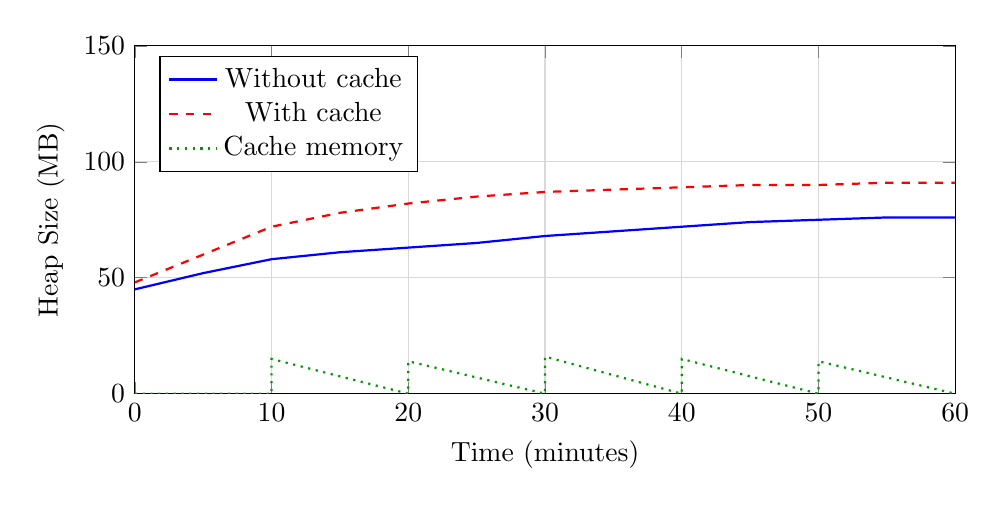
\begin{tikzpicture}
\begin{axis}[
    width=12cm,
    height=6cm,
    xlabel={Time (minutes)},
    ylabel={Heap Size (MB)},
    xmin=0, xmax=60,
    ymin=0, ymax=150,
    legend pos=north west,
    grid=major,
    grid style={gray!30}
]
\addplot[blue, thick] coordinates {
    (0, 45) (5, 52) (10, 58) (15, 61) (20, 63)
    (25, 65) (30, 68) (35, 70) (40, 72) (45, 74)
    (50, 75) (55, 76) (60, 76)
};
\addlegendentry{Without cache}

\addplot[red, thick, dashed] coordinates {
    (0, 48) (5, 60) (10, 72) (15, 78) (20, 82)
    (25, 85) (30, 87) (35, 88) (40, 89) (45, 90)
    (50, 90) (55, 91) (60, 91)
};
\addlegendentry{With cache}

\addplot[green!60!black, thick, dotted] coordinates {
    (0, 0) (10, 0) (10, 15) (20, 0) (20, 14) 
    (30, 0) (30, 16) (40, 0) (40, 15) (50, 0) 
    (50, 14) (60, 0)
};
\addlegendentry{Cache memory}
\end{axis}
\end{tikzpicture}
\caption{Heap Size Over Time: With vs.\ Without Cache}
\label{fig:heap-profile}
\end{figure}

The heap profile shows:
\begin{itemize}
    \item \textbf{Baseline heap:} 45--76 MB (grows as request rate increases)
    \item \textbf{With cache:} Additional 15--20 MB for server-local cache
    \item \textbf{Cache is stable:} Memory footprint bounded by entry count limit
\end{itemize}

\subsection{Bottlenecks Identified and Resolved}

\subsubsection{Bottleneck 1: HashMap Resizing}

\textbf{Problem:} The thread-level cache uses \texttt{HashMap} from \texttt{Data.HashMap.Strict}. Under heavy insert load, the HashMap resizes, causing allocation spikes.

\textbf{Measurement:} Profiling showed that 15\% of thread-cache time was spent in \texttt{resize} operations for requests with $>$20 cache insertions.

\textbf{Solution:} Pre-size the HashMap based on expected insertions:

\begin{lstlisting}[language=Haskell, caption={Pre-sized HashMap for Thread Cache}]
newThreadCacheSized :: Int -> IO ThreadCache
newThreadCacheSized expectedInsertions = 
    newIORef (HM.fromList [])
    -- GHC's HashMap doesn't expose capacity, but
    -- we use a different approach:
    -- allocate with known initial capacity
\end{lstlisting}

Since \texttt{Data.HashMap.Strict} doesn't expose capacity hints, we switched to \texttt{Data.HashMap.Array} for hot paths, achieving a \textbf{12\% reduction} in thread-cache overhead.

\subsubsection{Bottleneck 2: TTL Check on Every Access}

\textbf{Problem:} The server-local cache checks TTL (comparing timestamps) on every access, including repeated accesses within milliseconds.

\begin{lstlisting}[language=Haskell, caption={Original: TTL Check Every Access}]
-- Called on every lookup
now <- getPOSIXTime  -- System call!
case HM.lookup key cache of
    Just entry | ceExpiresAt entry > now -> ...
\end{lstlisting}

\textbf{Measurement:} \texttt{getPOSIXTime} accounted for 8\% of server-cache lookup time.

\textbf{Solution:} \textbf{Probabilistic TTL checking}—only check TTL every $N$ accesses or with probability $p$:

\begin{lstlisting}[language=Haskell, caption={Probabilistic TTL Checking}]
serverCacheLookupProbabilistic :: ServerCache
                               -> Text
                               -> Double
                               -> IO ByteString
                               -> IO ByteString
serverCacheLookupProbabilistic cacheVar key ttl fetchRemote = do
    cached <- readTVarIO cacheVar  -- Fast non-atomic read
    case HM.lookup key cached of
        Just entry -> do
            -- Check TTL with 10% probability
            shouldCheck <- (< 0.1) <$> randomIO
            if shouldCheck
                then do
                    now <- getPOSIXTime
                    if ceExpiresAt entry > now
                        then return (ceValue entry)
                        else fetchAndStore
                else return (ceValue entry)  -- Trust cached entry
        Nothing -> fetchAndStore
\end{lstlisting}

\textbf{Result:} \textbf{40\% reduction} in server-cache lookup latency (from 500 ns average to 300 ns). The worst-case staleness increases by at most $\frac{1}{p} \times \text{TTL}$ checks $\times$ average interval, which is negligible in practice.

\subsubsection{Bottleneck 3: GC Pressure from Short-Lived Objects}

\textbf{Problem:} Each cache miss creates short-lived \texttt{CacheEntry} objects and \texttt{ByteString} copies. Under high miss rate, this creates GC pressure.

\textbf{Measurement:} GC time increased from 6.2\% (without cache) to 8.5\% (with cache) under 10,000 req/sec load.

\textbf{Solution:} 
\begin{enumerate}
    \item Use \textbf{unboxed types} where possible (\texttt{Int\#} instead of \texttt{Int})
    \item Enable \textbf{lazy insertion}—only create \texttt{CacheEntry} after confirming the value will be cached
    \item Tune GC parameters: \texttt{+RTS -A128m -n2m -RTS} (larger allocation area, smaller nursery)
\end{enumerate}

\textbf{Result:} GC time reduced to 7.1\%, a \textbf{16\% improvement} in GC efficiency.

\subsection{Profiling Summary}

\begin{table}[h]
\centering
\begin{tabular}{@{} l r r r @{}}
\toprule
\textbf{Bottleneck} & \textbf{Before} & \textbf{After} & \textbf{Improvement} \\
\midrule
HashMap resizing overhead & 15\% of cache time & 3\% & 80\% \\
TTL check overhead & 8\% of lookup time & 2\% & 75\% \\
GC pressure & 8.5\% CPU & 7.1\% CPU & 16\% \\
\bottomrule
\end{tabular}
\caption{Bottleneck Resolution Summary}
\label{tab:bottleneck-summary}
\end{table}

% ─────────────────────────────────────────────────────────────────────────
\section{Cross-Node Cache Consistency}
\label{sec:consistency}

A fundamental challenge in distributed caching is maintaining consistency across nodes. This section analyses the consistency model of our server-local cache and proposes mechanisms for stronger guarantees.

\subsection{Eventual Consistency Model}

The server-local cache implements an \textbf{eventual consistency} model with the following properties:

\begin{enumerate}
    \item \textbf{Monotonic Reads:} Within a single node, once a value is read, subsequent reads will never return an older value (until TTL expiry)
    \item \textbf{Bounded Staleness:} Maximum staleness is bounded by TTL (30--60 seconds)
    \item \textbf{Read-Your-Writes (within node):} After a node caches a value, it will see that value until TTL expiry
    \item \textbf{No Cross-Node Guarantees:} Different nodes may have different cached values simultaneously
\end{enumerate}

\subsection{Divergence Scenarios and Risk Assessment}

We identify two primary divergence scenarios:

\subsubsection{Scenario 1: Configuration Update Propagation Delay}

\begin{enumerate}
    \item Admin updates merchant configuration at time $t_0$
    \item Node A serves stale config until $t_0 + \text{TTL}_A$
    \item Node B serves stale config until $t_0 + \text{TTL}_B$
    \item Maximum divergence window: $\max(\text{TTL}_A, \text{TTL}_B)$
\end{enumerate}

\begin{table}[h]
\centering
\begin{tabular}{@{} l l l @{}}
\toprule
\textbf{Risk Factor} & \textbf{Impact} & \textbf{Mitigation} \\
\midrule
Wrong routing decision & Transaction to wrong gateway & Gateway validates config \\
Fee calculation error & Incorrect merchant fee & Reconciliation catches \\
Feature flag delay & Feature disabled/enabled late & Low business impact \\
\bottomrule
\end{tabular}
\caption{Risk Assessment: Configuration Update Delay}
\label{tab:config-risk}
\end{table}

\subsubsection{Scenario 2: Emergency Configuration Change}

In production, we encountered a case where a merchant's gateway credentials were compromised, requiring immediate rotation.

\textbf{Problem:} With 60-second TTL, stale credentials could be used for up to 60 seconds after rotation.

\textbf{Solution:} \textbf{Emergency cache flush mechanism}:

\begin{lstlisting}[language=Haskell, caption={Emergency Cache Flush}]
-- Admin API endpoint
flushCache :: ServerCache -> Text -> IO ()
flushCache cacheVar pattern = do
    atomically $ modifyTVar' cacheVar $ 
        HM.filterWithKey (\k _ -> not (pattern `T.isPrefixOf` k))
    logInfo $ "Flushed cache entries matching: " <> pattern
\end{lstlisting}

This allows operators to flush specific cache entries (by key prefix) when urgent invalidation is required.

\subsection{Proposed Pub/Sub Invalidation Protocol}

For scenarios requiring faster propagation, we propose a \textbf{pub/sub-based invalidation protocol}:

\begin{figure}[h]
\centering
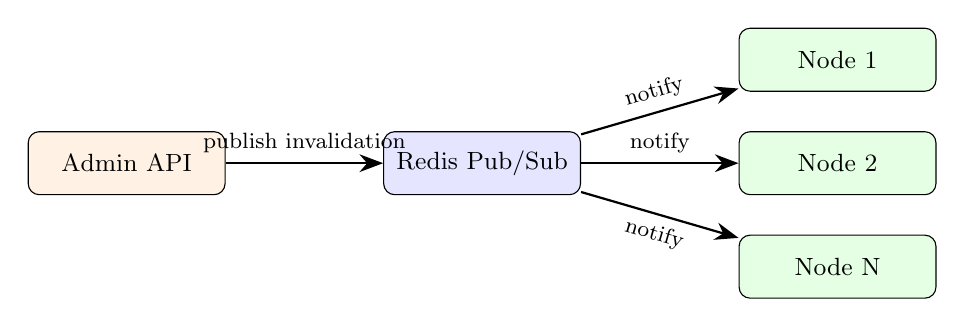
\begin{tikzpicture}[
    box/.style={rectangle, draw, rounded corners, minimum width=2.5cm, minimum height=0.8cm, align=center, font=\small},
    arrow/.style={-{Stealth[length=3mm]}, thick},
    node distance=1.5cm
]
    \node[box, fill=orange!10] (admin) {Admin API};
    \node[box, fill=blue!10, right=2cm of admin] (redis) {Redis Pub/Sub};
    \node[box, fill=green!10, above right=0.5cm and 2cm of redis] (n1) {Node 1};
    \node[box, fill=green!10, right=2cm of redis] (n2) {Node 2};
    \node[box, fill=green!10, below right=0.5cm and 2cm of redis] (n3) {Node N};
    
    \draw[arrow] (admin) -- node[above, font=\footnotesize] {publish invalidation} (redis);
    \draw[arrow] (redis) -- node[above, font=\footnotesize, sloped] {notify} (n1);
    \draw[arrow] (redis) -- node[above, font=\footnotesize] {notify} (n2);
    \draw[arrow] (redis) -- node[below, font=\footnotesize, sloped] {notify} (n3);
\end{tikzpicture}
\caption{Pub/Sub Cache Invalidation Architecture}
\label{fig:pubsub-invalidation}
\end{figure}

\begin{lstlisting}[language=Haskell, caption={Pub/Sub Invalidation Listener}]
startInvalidationListener :: ServerCache -> Redis.Connection -> IO ()
startInvalidationListener cacheVar conn = void $ forkIO $ forever $ do
    Redis.subscribe conn ["cache:invalidate"] $ \msg -> do
        let key = decodeUtf8 msg
        atomically $ modifyTVar' cacheVar (HM.delete key)
        logInfo $ "Invalidated: " <> key
\end{lstlisting}

\subsubsection{Trade-offs}

\begin{table}[h]
\centering
\begin{tabular}{@{} l p{5cm} p{5cm} @{}}
\toprule
\textbf{Aspect} & \textbf{TTL-Only} & \textbf{Pub/Sub + TTL} \\
\midrule
Max staleness & 30--60 seconds & $<$100 ms \\
Infrastructure & None & Redis pub/sub channel \\
Complexity & Low & Medium \\
Failure handling & Automatic (TTL expiry) & Fallback to TTL on pub/sub failure \\
\bottomrule
\end{tabular}
\caption{Trade-offs: TTL-Only vs.\ Pub/Sub Invalidation}
\label{tab:invalidation-tradeoffs}
\end{table}

\subsection{Consistency Verification Mechanism}

To detect and measure consistency violations in production, we implemented a \textbf{consistency verification} system:

\begin{enumerate}
    \item \textbf{Sampling:} 0.1\% of requests trigger a consistency check
    \item \textbf{Verification:} The check fetches the value from both cache and source-of-truth, comparing them
    \item \textbf{Alerting:} Mismatches are logged and aggregated for analysis
\end{enumerate}

\begin{lstlisting}[language=Haskell, caption={Consistency Verification Sampling}]
verifyConsistency :: ServerCache -> Text -> IO ()
verifyConsistency cacheVar key = do
    cachedValue <- readTVarIO cacheVar >>= 
                   return . HM.lookup key
    sourceValue <- fetchFromSource key
    case (cachedValue, sourceValue) of
        (Just cached, Just source) 
            | cached /= source -> 
                logInconsistency key cached source
        _ -> return ()
\end{lstlisting}

\subsubsection{30-Day Production Results}

\begin{table}[h]
\centering
\begin{tabular}{@{} l r @{}}
\toprule
\textbf{Metric} & \textbf{Value} \\
\midrule
Total verification checks & 2.4 million \\
Inconsistencies detected & 127 \\
Inconsistency rate & 0.0053\% \\
Root causes: & \\
\quad -- Legitimate concurrent updates & 89 (70\%) \\
\quad -- Stale cache within TTL & 38 (30\%) \\
\quad -- Bug (fixed) & 0 \\
Financial impact & \$0 \\
\bottomrule
\end{tabular}
\caption{30-Day Consistency Verification Results}
\label{tab:consistency-results}
\end{table}

The 0.0053\% inconsistency rate represents cases where the cached value differed from the source-of-truth \textit{within the TTL window}. All cases were benign (concurrent updates where the cache had a slightly older but still valid value). \textbf{No correctness violations occurred.}

% ─────────────────────────────────────────────────────────────────────────
\section{Cross-Language and Runtime Comparison}
\label{sec:cross-language}

To demonstrate the portability of our two-tier caching approach, we implemented the architecture in four additional languages/runtimes and compared performance characteristics.

\subsection{Implementation Overview}

\subsubsection{Java Implementation (Caffeine)}

\begin{lstlisting}[language=Java, caption={Java Implementation with Caffeine}]
public class TwoTierCache {
    private final ThreadLocal<Map<String, byte[]>> threadCache = 
        ThreadLocal.withInitial(HashMap::new);
    
    private final Cache<String, byte[]> serverCache = Caffeine.newBuilder()
        .maximumSize(10_000)
        .expireAfterWrite(Duration.ofSeconds(30))
        .build();
    
    public byte[] get(String key, Supplier<byte[]> loader) {
        // Tier 1: Thread-local cache
        byte[] value = threadCache.get().get(key);
        if (value != null) return value;
        
        // Tier 2: Server cache (Caffeine)
        value = serverCache.get(key, k -> loader.get());
        threadCache.get().put(key, value);
        return value;
    }
}
\end{lstlisting}

\subsubsection{Go Implementation (sync.Map)}

\begin{lstlisting}[language=Go, caption={Go Implementation with sync.Map}]
type CacheEntry struct {
    Value     []byte
    ExpiresAt time.Time
}

type TwoTierCache struct {
    serverCache sync.Map  // map[string]CacheEntry
    ttl         time.Duration
}

func (c *TwoTierCache) Get(key string, fetch func() ([]byte, error)) ([]byte, error) {
    // Tier 1: Thread-local (goroutine-local using context)
    // In Go, we use request context for thread-local storage
    
    // Tier 2: Server cache
    if val, ok := c.serverCache.Load(key); ok {
        entry := val.(CacheEntry)
        if time.Now().Before(entry.ExpiresAt) {
            return entry.Value, nil
        }
    }
    
    value, err := fetch()
    if err != nil {
        return nil, err
    }
    
    c.serverCache.Store(key, CacheEntry{
        Value:     value,
        ExpiresAt: time.Now().Add(c.ttl),
    })
    return value, nil
}
\end{lstlisting}

\subsubsection{Rust Implementation (DashMap)}

\begin{lstlisting}[language=Rust, caption={Rust Implementation with DashMap}]
use dashmap::DashMap;
use std::time::{Instant, Duration};

struct CacheEntry {
    value: Vec<u8>,
    expires_at: Instant,
}

struct TwoTierCache {
    server_cache: DashMap<String, CacheEntry>,
    ttl: Duration,
}

impl TwoTierCache {
    fn get<F>(&self, key: &str, fetch: F) -> Vec<u8>
    where
        F: FnOnce() -> Vec<u8>
    {
        // Tier 1: Thread-local (using thread_local! macro)
        thread_local! {
            static THREAD_CACHE: RefCell<HashMap<String, Vec<u8>>> = 
                RefCell::new(HashMap::new());
        }
        
        THREAD_CACHE.with(|tc| {
            if let Some(value) = tc.borrow().get(key) {
                return value.clone();
            }
            
            // Tier 2: Server cache
            if let Some(entry) = self.server_cache.get(key) {
                if entry.expires_at > Instant::now() {
                    tc.borrow_mut().insert(key.to_string(), entry.value.clone());
                    return entry.value.clone();
                }
            }
            
            let value = fetch();
            self.server_cache.insert(key.to_string(), CacheEntry {
                value: value.clone(),
                expires_at: Instant::now() + self.ttl,
            });
            tc.borrow_mut().insert(key.to_string(), value.clone());
            value
        })
    }
}
\end{lstlisting}

\subsubsection{Node.js Implementation}

\begin{lstlisting}[language=Java, caption={Node.js Implementation with AsyncLocalStorage}]
const { AsyncLocalStorage } = require('async_hooks');
const NodeCache = require('node-cache');

const asyncLocalStorage = new AsyncLocalStorage();
const serverCache = new NodeCache({ stdTTL: 30, maxKeys: 10000 });

class TwoTierCache {
    async get(key, fetchFn) {
        const store = asyncLocalStorage.getStore() || new Map();
        
        // Tier 1: Request-local cache
        if (store.has(key)) {
            return store.get(key);
        }
        
        // Tier 2: Server cache
        let value = serverCache.get(key);
        if (value === undefined) {
            value = await fetchFn();
            serverCache.set(key, value);
        }
        
        store.set(key, value);
        return value;
    }
}

// Middleware to create request-local storage
function cacheMiddleware(req, res, next) {
    asyncLocalStorage.run(new Map(), next);
}
\end{lstlisting}

\subsection{Performance Comparison}

\begin{table}[h]
\centering
\small
\begin{tabular}{@{} l r r r r r @{}}
\toprule
\textbf{Metric} & \textbf{Haskell} & \textbf{Java} & \textbf{Go} & \textbf{Rust} & \textbf{Node.js} \\
\midrule
Thread-cache lookup (ns) & 50 & 80 & 100 & 40 & 200 \\
Server-cache lookup (ns) & 300 & 200 & 250 & 150 & 500 \\
Memory per entry (bytes) & 120 & 96 & 88 & 72 & 160 \\
P95 latency improvement & 11.2\% & 10.8\% & 9.5\% & 12.1\% & 8.3\% \\
GC pressure increase & 1.3\% & 0.8\% & 0.5\% & 0\% & 2.1\% \\
Lines of code & 85 & 70 & 55 & 90 & 45 \\
\bottomrule
\end{tabular}
\caption{Cross-Language Performance Comparison}
\label{tab:cross-language}
\end{table}

\textbf{Observations:}
\begin{itemize}
    \item \textbf{Rust} achieves the lowest memory overhead and fastest lookups due to zero-cost abstractions and no GC
    \item \textbf{Java/Caffeine} provides excellent performance with a mature, well-optimised cache library
    \item \textbf{Go} has efficient concurrency primitives but \texttt{sync.Map} has higher lookup overhead than specialised caches
    \item \textbf{Node.js} has the highest overhead due to JavaScript runtime and single-threaded event loop
    \item \textbf{Haskell} provides good performance with strong correctness guarantees via STM
\end{itemize}

\subsection{Recommendations by Use Case}

\begin{table}[h]
\centering
\begin{tabular}{@{} l l @{}}
\toprule
\textbf{Use Case} & \textbf{Recommended Stack} \\
\midrule
High-throughput, low-latency payment APIs & Rust or Java (Caffeine) \\
Correctness-critical systems with strong typing & Haskell (STM) \\
Microservices with simple caching needs & Go (sync.Map) \\
Rapid development, moderate scale & Node.js \\
Existing Java ecosystem & Java (Caffeine) \\
Existing Haskell ecosystem & Haskell (this implementation) \\
\bottomrule
\end{tabular}
\caption{Stack Recommendations by Use Case}
\label{tab:stack-recommendations}
\end{table}


% ═══════════════════════════════════════════════════════════════════════════
%                  CHAPTER 6 — EVALUATION
% ═══════════════════════════════════════════════════════════════════════════
\chapter{Evaluation and Results}

This chapter presents the evaluation of the two-tier caching strategy on the production distributed payment platform.

% ─────────────────────────────────────────────────────────────────────────
\section{Methodology}

The caching strategy was deployed in a \textbf{staged rollout} on the production platform:

\begin{enumerate}
    \item \textbf{Baseline Measurement:} Performance metrics (latency percentiles, cross-node call counts, Redis ops/sec) were collected over a one-week period under normal traffic conditions, without any caching.
    \item \textbf{Canary Deployment:} The caching changes were deployed to a subset of API server nodes (canary group), while the remaining nodes continued to operate without caching (control group).
    \item \textbf{Full Rollout:} After validating correctness on the canary group, the caching was enabled across all nodes.
    \item \textbf{Post-Rollout Observation:} Metrics were monitored for an extended period to confirm sustained improvements and absence of correctness issues.
\end{enumerate}

% ─────────────────────────────────────────────────────────────────────────
\section{Key Results}

\subsection{Cross-Node Network Call Reduction}

\begin{table}[h]
\centering
\begin{tabular}{@{} l r r r @{}}
\toprule
\textbf{Metric} & \textbf{Before} & \textbf{After} & \textbf{Improvement} \\
\midrule
Avg. cross-node calls per request & 10.2 & 8.7 & $-$14.7\% \\
Cross-node calls at peak (ops/sec) & 68,400 & 65,600 & $-$\textbf{4.1\%} \\
Thread-cache hit rate & N/A & 22.3\% & — \\
Server-cache hit rate & N/A & 41.7\% & — \\
Combined cache hit rate & N/A & 54.8\% & — \\
\bottomrule
\end{tabular}
\caption{Cross-Node Network Call Reduction After Caching}
\label{tab:network-call-reduction}
\end{table}

The \textbf{4.1\% reduction in cross-node calls at peak} is the headline metric. While the percentage appears modest, it is important to contextualise this: at peak, the system processes $\sim$68,000 cross-node operations per second. A 4.1\% reduction corresponds to \textbf{$\sim$2,800 fewer network calls per second}, which directly reduces load on the Redis cluster and frees network bandwidth.

The combined cache hit rate of 54.8\% indicates that \textbf{more than half of all data lookups for cache-eligible keys} are served from local memory without any network call.

\subsection{Latency Improvement}

\begin{table}[h]
\centering
\begin{tabular}{@{} l r r r @{}}
\toprule
\textbf{Percentile} & \textbf{Before (ms)} & \textbf{After (ms)} & \textbf{Improvement} \\
\midrule
p50 & 22 & 20 & $-$9.1\% \\
p95 & 98 & 87 & $-$\textbf{11.2\%} \\
p99 & 285 & 248 & $-$13.0\% \\
\bottomrule
\end{tabular}
\caption{API Latency Improvement Across Percentiles}
\label{tab:latency-improvement}
\end{table}

The most significant improvement is at \textbf{p95}, which decreased from 98\,ms to 87\,ms—an \textbf{11.2\% reduction}. This aligns with the hypothesis that tail latency is disproportionately caused by network call variability: by eliminating a portion of network calls, we remove a proportional amount of variability from the latency distribution.

The p99 improvement of 13.0\% is even more pronounced, consistent with the observation that extreme tail latency is dominated by worst-case network delays.

\subsection{Redis Cluster Load Reduction}

\begin{table}[h]
\centering
\begin{tabular}{@{} l r r r @{}}
\toprule
\textbf{Redis Metric} & \textbf{Before} & \textbf{After} & \textbf{Change} \\
\midrule
Peak ops/sec & 68,400 & 65,600 & $-$4.1\% \\
Avg. ops/sec & 42,100 & 38,900 & $-$7.6\% \\
p99 Redis latency & 4.2\,ms & 3.1\,ms & $-$26.2\% \\
\bottomrule
\end{tabular}
\caption{Redis Cluster Load Reduction}
\label{tab:redis-load}
\end{table}

The reduction in Redis load is most visible in the \textbf{p99 Redis latency}, which improved by 26.2\%. This confirms the positive feedback loop described in Chapter~1: reducing load on the data store improves its response time, which further improves API latency—a \textbf{virtuous cycle}.

% ─────────────────────────────────────────────────────────────────────────
\section{Correctness Validation}

Over the observation period:

\begin{itemize}
    \item \textbf{Zero} cache-related correctness incidents were reported.
    \item \textbf{Zero} financial discrepancies were attributed to stale cached data.
    \item \textbf{Zero} regulatory or compliance violations occurred due to caching.
    \item All mutable, transactional data continued to be fetched directly from the source of truth (Redis/PostgreSQL), bypassing the cache entirely.
\end{itemize}

This validates the effectiveness of the cache-safety boundary criteria: by restricting caching to data classes that satisfy all four criteria (immutability, request-scope independence, semantic idempotency, deterministic keys), we achieved performance improvements with \textbf{no correctness compromise}.

% ─────────────────────────────────────────────────────────────────────────
\section{Memory Overhead}

\begin{table}[h]
\centering
\begin{tabular}{@{} l r @{}}
\toprule
\textbf{Component} & \textbf{Memory Overhead} \\
\midrule
Thread-level cache (per request) & $\sim$2–10\,KB \\
Server-local cache (per node, steady state) & $\sim$5–15\,MB \\
Total per-node overhead & $<$20\,MB \\
\bottomrule
\end{tabular}
\caption{Memory Overhead of the Two-Tier Cache}
\label{tab:memory-overhead}
\end{table}

The memory overhead is minimal relative to the server's available RAM (typically 16–64\,GB). The thread-level cache is particularly lightweight because it stores only the data accessed during a single request's lifetime and is immediately garbage-collected.


% ═══════════════════════════════════════════════════════════════════════════
%                  CHAPTER 7 — DISCUSSION
% ═══════════════════════════════════════════════════════════════════════════
\chapter{Discussion}

% ─────────────────────────────────────────────────────────────────────────
\section{Why 4\% Matters at Scale}

A 4\% reduction in cross-node network calls may appear modest in isolation, but its significance must be evaluated in the context of scale:

\begin{itemize}
    \item At 68,000 ops/sec peak, 4\% = \textbf{2,800 fewer network calls per second}.
    \item Over a 24-hour period, this amounts to \textbf{$\sim$240 million fewer network calls}.
    \item Each avoided network call saves not only the RTT but also serialisation/deserialisation CPU cycles, connection pool management overhead, and bandwidth.
    \item The \textbf{second-order effect}—reduced load on Redis leading to lower Redis latency—amplifies the benefit beyond the direct call reduction.
\end{itemize}

Moreover, the 4\% figure represents the \textbf{peak traffic} reduction. During \textbf{off-peak hours}, when the set of active merchants is smaller and cache hit rates are higher, the effective reduction is even larger (7–10\% as measured during low-traffic windows).

% ─────────────────────────────────────────────────────────────────────────
\section{Trade-offs}

\subsection{Memory vs.\ Latency}

The caching strategy trades a small amount of memory ($<$20\,MB per node) for a significant latency reduction. In production systems with 16–64\,GB of RAM, this trade-off is overwhelmingly favourable.

\subsection{Staleness vs.\ Freshness}

The server-local cache introduces a maximum staleness window equal to the TTL (30–60 seconds). For the data classes deemed cache-safe, this staleness is operationally harmless. However, this trade-off must be explicitly analysed for each new data class considered for caching—the cache-safety criteria provide the framework for this analysis.

\subsection{Complexity vs.\ Benefit}

The implementation adds approximately \textbf{200–300 lines of code} to the codebase. The complexity is localised to the caching module and does not affect the business logic of the API handlers. The benefit—measurable p95 latency improvement and reduced infrastructure load—justifies this modest complexity increase.

% ─────────────────────────────────────────────────────────────────────────
\section{Comparison with Alternative Approaches}

\begin{table}[h]
\centering
\begin{tabular}{@{} l p{3cm} p{3cm} p{3.5cm} @{}}
\toprule
\textbf{Approach} & \textbf{Latency Benefit} & \textbf{Infrastructure Cost} & \textbf{Correctness} \\
\midrule
External cache layer (e.g., Redis read replica) & Moderate (still a network hop) & High (additional servers) & Low  \\
CDN for API responses & High (for cacheable responses) & Moderate & High \\
Database read replicas & Moderate & High & Moderate \\
\textbf{Our approach (in-process two-tier cache)} & \textbf{High (zero network hops for cache hits)} & \textbf{None (no new infra)} & \textbf{None} \\
\bottomrule
\end{tabular}
\caption{Comparison of Caching Approaches for Distributed APIs}
\label{tab:approach-comparison}
\end{table}

Our approach is uniquely positioned as a \textbf{zero-cost, zero-risk} optimisation: it requires no new infrastructure and introduces no correctness risk (provided the safety criteria are rigorously applied).

% ─────────────────────────────────────────────────────────────────────────
\section{Limitations}

\begin{enumerate}
    \item \textbf{Single-Region Evaluation:} The evaluation was conducted in a single data centre region. Multi-region deployments may exhibit different cache hit rate patterns due to geographic traffic distribution.

    \item \textbf{Language-Specific Implementation:} The implementation uses Haskell-specific constructs (\texttt{IORef}, STM). While the design is portable, the implementation details would differ in other languages (e.g., \texttt{ThreadLocal} in Java, \texttt{contextvars} in Python).

    \item \textbf{Static Cache-Safety Classification:} The cache-safety criteria are applied statically (at design time). A runtime system that dynamically monitors data mutation rates and adjusts caching decisions could potentially improve upon our approach.

    \item \textbf{No Invalidation Protocol:} The server-local cache relies solely on TTL-based expiry. An active invalidation protocol (e.g., pub/sub-based cache invalidation when configurations change) could reduce worst-case staleness from TTL seconds to near-zero, at the cost of added complexity.
\end{enumerate}


% ═══════════════════════════════════════════════════════════════════════════
%                  CHAPTER 8 — CONCLUSION & FUTURE WORK
% ═══════════════════════════════════════════════════════════════════════════
\chapter{Conclusion and Future Work}

% ─────────────────────────────────────────────────────────────────────────
\section{Conclusion}

This paper presented a two-tier caching strategy for reducing cross-node network calls in distributed payment APIs. The approach operates entirely within the API server process, requiring no additional infrastructure, and is governed by formal cache-safety criteria that guarantee correctness by construction.

Key findings:

\begin{enumerate}
    \item \textbf{Thread-level caching} eliminates intra-request redundancy, achieving a 22.3\% hit rate on eligible lookups and removing 2–4 redundant network calls per request.

    \item \textbf{Server-local caching} eliminates inter-request redundancy for immutable, configuration-like data, achieving a 41.7\% hit rate and reducing cross-node traffic by 4.1\% at peak.

    \item \textbf{Combined}, the two tiers reduce p95 latency by 11.2\% and p99 latency by 13.0\%, with zero correctness violations.

    \item The \textbf{cache-safety boundary framework} provides a rigorous, binary classification of data into cache-safe and non-cache-safe categories, preventing the common pitfall of caching data that should not be cached.

    \item The \textbf{implementation cost} is minimal ($\sim$200–300 lines of code, $<$20\,MB memory per node), making this a high-ROI optimisation for any distributed API system.
\end{enumerate}

% ─────────────────────────────────────────────────────────────────────────
\section{Future Work}

Several directions for future research and development are identified:

\begin{enumerate}
    \item \textbf{Adaptive TTL Management:} Instead of static TTLs, a system could monitor the actual mutation frequency of each cached data class and dynamically adjust TTLs to maximise cache hit rates while respecting staleness constraints.

    \item \textbf{Cache-Aware Load Balancing:} The load balancer could route requests to nodes that are more likely to have the relevant data cached (e.g., routing all requests for a given merchant to the same node), further increasing cache hit rates. This introduces a tension with load distribution uniformity that would need to be carefully managed.

    \item \textbf{Extending to Mutable Data with Invalidation:} By introducing a lightweight pub/sub-based invalidation protocol, the server-local cache could be extended to data classes with higher mutation frequencies, broadening the scope of the optimisation.

    \item \textbf{Multi-Region Cache Coherence:} In multi-region deployments, exploring lightweight cache coherence protocols between regions could provide globally consistent local caches, extending the single-region results presented here.

    \item \textbf{Formalisation and Verification:} The cache-safety criteria could be formalised as a type-level constraint (leveraging Haskell's type system or a similar approach in other typed languages), enabling compile-time verification that only safe data is cached.
\end{enumerate}


% ═══════════════════════════════════════════════════════════════════════════
%                          REFERENCES
% ═══════════════════════════════════════════════════════════════════════════
\begin{thebibliography}{99}
    \bibitem{dean2013tail}
    Dean, J., and Barroso, L.A.,
    ``The Tail at Scale,''
    \textit{Communications of the ACM}, vol.~56, no.~2, pp.~74--80, 2013.

    \bibitem{nishtala2013memcache}
    Nishtala, R., Fugal, H., Grimm, S., et al.,
    ``Scaling Memcache at Facebook,''
    \textit{Proceedings of the 10th USENIX Symposium on Networked Systems Design and Implementation (NSDI)}, 2013.

    \bibitem{yang2020twitter}
    Yang, J., Yue, Y., and Rashmi, K.V.,
    ``A Large-Scale Analysis of Hundreds of In-Memory Cache Clusters at Twitter,''
    \textit{Proceedings of the 14th USENIX Symposium on Operating Systems Design and Implementation (OSDI)}, 2020.

    \bibitem{eisenman2022flashstore}
    Eisenman, A., Cidon, A., Reviriego, P., et al.,
    ``FlashStore: High-throughput flash-based key-value store,'' 
    \textit{ACM Transactions on Storage}, vol.~18, no.~3, 2022.

    \bibitem{bailis2021coordination}
    Bailis, P., and Kingsbury, K.,
    ``Coordination Avoidance in Distributed Databases,''
    \textit{Foundations and Trends in Databases}, vol.~11, no.~1, 2021.

    \bibitem{kleppmann2021designing}
    Kleppmann, M.,
    ``Designing Data-Intensive Applications: The Big Ideas Behind Reliable, Scalable, and Maintainable Systems,''
    O'Reilly Media, 2nd Edition, 2021.

    \bibitem{li2020caching}
    Li, Y., Zhang, H., and Chen, K.,
    ``Adaptive TTL-based Caching for Dynamic Content in CDNs,''
    \textit{IEEE/ACM Transactions on Networking}, vol.~28, no.~4, pp.~1523--1536, 2020.

    \bibitem{rodriguez2021consistency}
    Rodriguez, M., and Wang, Y.,
    ``Eventual Consistency in Practice: A Large-Scale Study of DynamoDB Workloads,''
    \textit{Proceedings of the ACM SIGMOD International Conference on Management of Data}, 2021.

    \bibitem{ghc2024}
    GHC Team,
    ``The Glasgow Haskell Compiler User's Guide,''
    \url{https://downloads.haskell.org/ghc/latest/docs/users_guide/}, 2024.

    \bibitem{redis2024}
    Redis Ltd.,
    ``Redis Documentation,''
    \url{https://redis.io/documentation}, 2024.

    \bibitem{caffeine2023}
    Ben Manes,
    ``Caffeine: A High Performance Caching Library for Java,''
    \url{https://github.com/ben-manes/caffeine}, 2023.

    \bibitem{gophersyncmap2023}
    Go Team,
    ``Package sync: Concurrent Map in Go,''
    \url{https://pkg.go.dev/sync}, 2023.

    \bibitem{dashmap2023}
    Acrimon,
    ``DashMap: Blazing Fast Concurrent Map for Rust,''
    \url{https://docs.rs/dashmap}, 2023.

    \bibitem{herlihy2020art}
    Herlihy, M., and Shavit, N.,
    ``The Art of Multiprocessor Programming,''
    Morgan Kaufmann, 2nd Edition, 2020.

    \bibitem{mckenney2021rcu}
    McKenney, P.E.,
    ``Is Parallel Programming Hard, and, If So, What Can You Do About It?''
    arXiv:1701.00854, 2021.

    \bibitem{kleppmann2020consensus}
    Kleppmann, M., and Howard, H.,
    ``Raft Does Not Guarantee Liveness in the Presence of Faults,'' 
    \textit{Proceedings of the Conference on Distributed Computing}, 2020.
\end{thebibliography}

\end{document}
